\section{eo\-VRPStat Class Reference}
\label{classeo_v_r_p_stat}\index{eoVRPStat@{eoVRPStat}}
Manages the statistics of the VRP problem.  


{\tt \#include $<$eo\-VRPStat.h$>$}

Inheritance diagram for eo\-VRPStat::\begin{figure}[H]
\begin{center}
\leavevmode
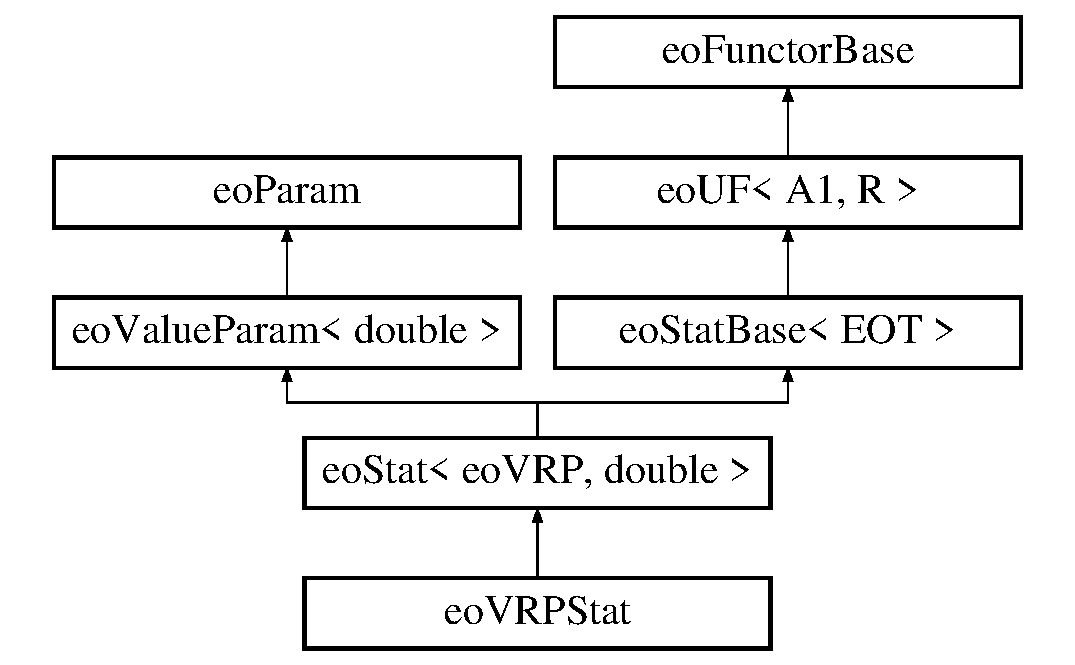
\includegraphics[height=5cm]{classeo_v_r_p_stat}
\end{center}
\end{figure}
\subsection*{Public Member Functions}
\begin{CompactItemize}
\item 
\bf{eo\-VRPStat} (std::string \_\-description=\char`\"{}eo\-VRPStat \char`\"{})
\begin{CompactList}\small\item\em Constructor: initializes variables properly. \item\end{CompactList}\item 
void \bf{operator()} (const \bf{eo\-Pop}$<$ \bf{eo\-VRP} $>$ \&\_\-pop)
\begin{CompactList}\small\item\em Gets statistics from a population. \item\end{CompactList}\item 
virtual std::string \bf{class\-Name} (void) const 
\begin{CompactList}\small\item\em Returns a string containing the name of the class. \item\end{CompactList}\end{CompactItemize}


\subsection{Detailed Description}
Manages the statistics of the VRP problem. 



Definition at line 47 of file eo\-VRPStat.h.

\subsection{Constructor \& Destructor Documentation}
\index{eoVRPStat@{eo\-VRPStat}!eoVRPStat@{eoVRPStat}}
\index{eoVRPStat@{eoVRPStat}!eoVRPStat@{eo\-VRPStat}}
\subsubsection{\setlength{\rightskip}{0pt plus 5cm}eo\-VRPStat::eo\-VRPStat (std::string {\em \_\-description} = {\tt \char`\"{}eoVRPStat~\char`\"{}})\hspace{0.3cm}{\tt  [inline]}}\label{classeo_v_r_p_stat_a326e09d7efebb4c572ea51ae517e058}


Constructor: initializes variables properly. 

\begin{Desc}
\item[Parameters:]
\begin{description}
\item[{\em \_\-description}]A string identifying the class. \end{description}
\end{Desc}


Definition at line 56 of file eo\-VRPStat.h.

\subsection{Member Function Documentation}
\index{eoVRPStat@{eo\-VRPStat}!operator()@{operator()}}
\index{operator()@{operator()}!eoVRPStat@{eo\-VRPStat}}
\subsubsection{\setlength{\rightskip}{0pt plus 5cm}void eo\-VRPStat::operator() (const \bf{eo\-Pop}$<$ \bf{eo\-VRP} $>$ \& {\em \_\-pop})\hspace{0.3cm}{\tt  [inline]}}\label{classeo_v_r_p_stat_5e773fab9c82e0a06d075af4be265d1e}


Gets statistics from a population. 

\begin{Desc}
\item[Parameters:]
\begin{description}
\item[{\em \_\-pop}]The population that will be analyzed. \end{description}
\end{Desc}


Definition at line 66 of file eo\-VRPStat.h.

References eo\-Value\-Param$<$ T $>$::value().\index{eoVRPStat@{eo\-VRPStat}!className@{className}}
\index{className@{className}!eoVRPStat@{eo\-VRPStat}}
\subsubsection{\setlength{\rightskip}{0pt plus 5cm}virtual std::string eo\-VRPStat::class\-Name (void) const\hspace{0.3cm}{\tt  [inline, virtual]}}\label{classeo_v_r_p_stat_61d9ece1bde19f4cd997c3aba075d8e7}


Returns a string containing the name of the class. 

Used to display statistics. \begin{Desc}
\item[Returns:]The string containing the name of the class. \end{Desc}


Reimplemented from \bf{eo\-Stat$<$ eo\-VRP, double $>$}.

Definition at line 79 of file eo\-VRPStat.h.

The documentation for this class was generated from the following file:\begin{CompactItemize}
\item 
eo\-VRPStat.h\end{CompactItemize}
